Underwater imaging has long been crucial in various fields, such as marine research, environmental monitoring, underwater archaeology, and offshore industries. Underwater imaging has long been crucial in various fields, such as marine research, environmental monitoring, underwater archaeology, and offshore industries. For example, scientists use underwater photography with quadrats to audit the abundance of coral over time at several reef locations \cite{universityofhawaiiPracticesScienceUnderwater}. Unmanned Underwater Vehicles (UUVs), a type of submersible vehicle, are pivotal in advancing underwater imaging capabilities. Often housing vast arrays of sophisticated sensors, these vehicles enable the end user to explore and analyse underwater environments with unprecedented accuracy and efficiency. Their autonomous or remote-controlled nature advocates the ideal platform for conducting missions of extended duration in hazardous conditions, impossible for direct human presence and intervention. With the benefits of UUV deployment, they have become common as a safer and cheaper alternative to manned vehicular operations in the vast range of underwater imaging-related industries and applications, such as intelligence surveillance and reconnaissance in defence, inspection and identification of defects or foreign objects in maritime, and oceanography and hydrography in marine research \cite{yannickallardUnmannedUnderwaterVehicle2014}.

\begin{figure}[h]
    \centering
    \begin{subfigure}{.25\textwidth}
        \centering
        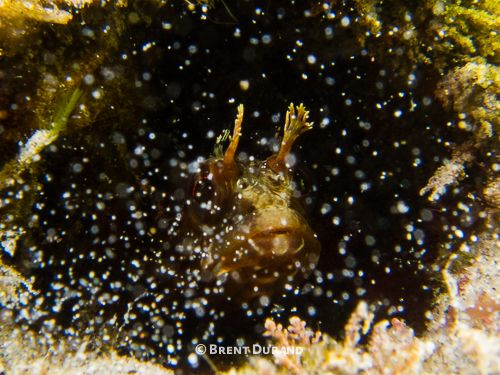
\includegraphics[width=1\linewidth]{assets/backscatter_article_durand2.jpg}
        \caption{}
        % \label{subfig:backscatter_durand}
    \end{subfigure}
    \qquad
    \begin{subfigure}{.34\textwidth}
        \centering
        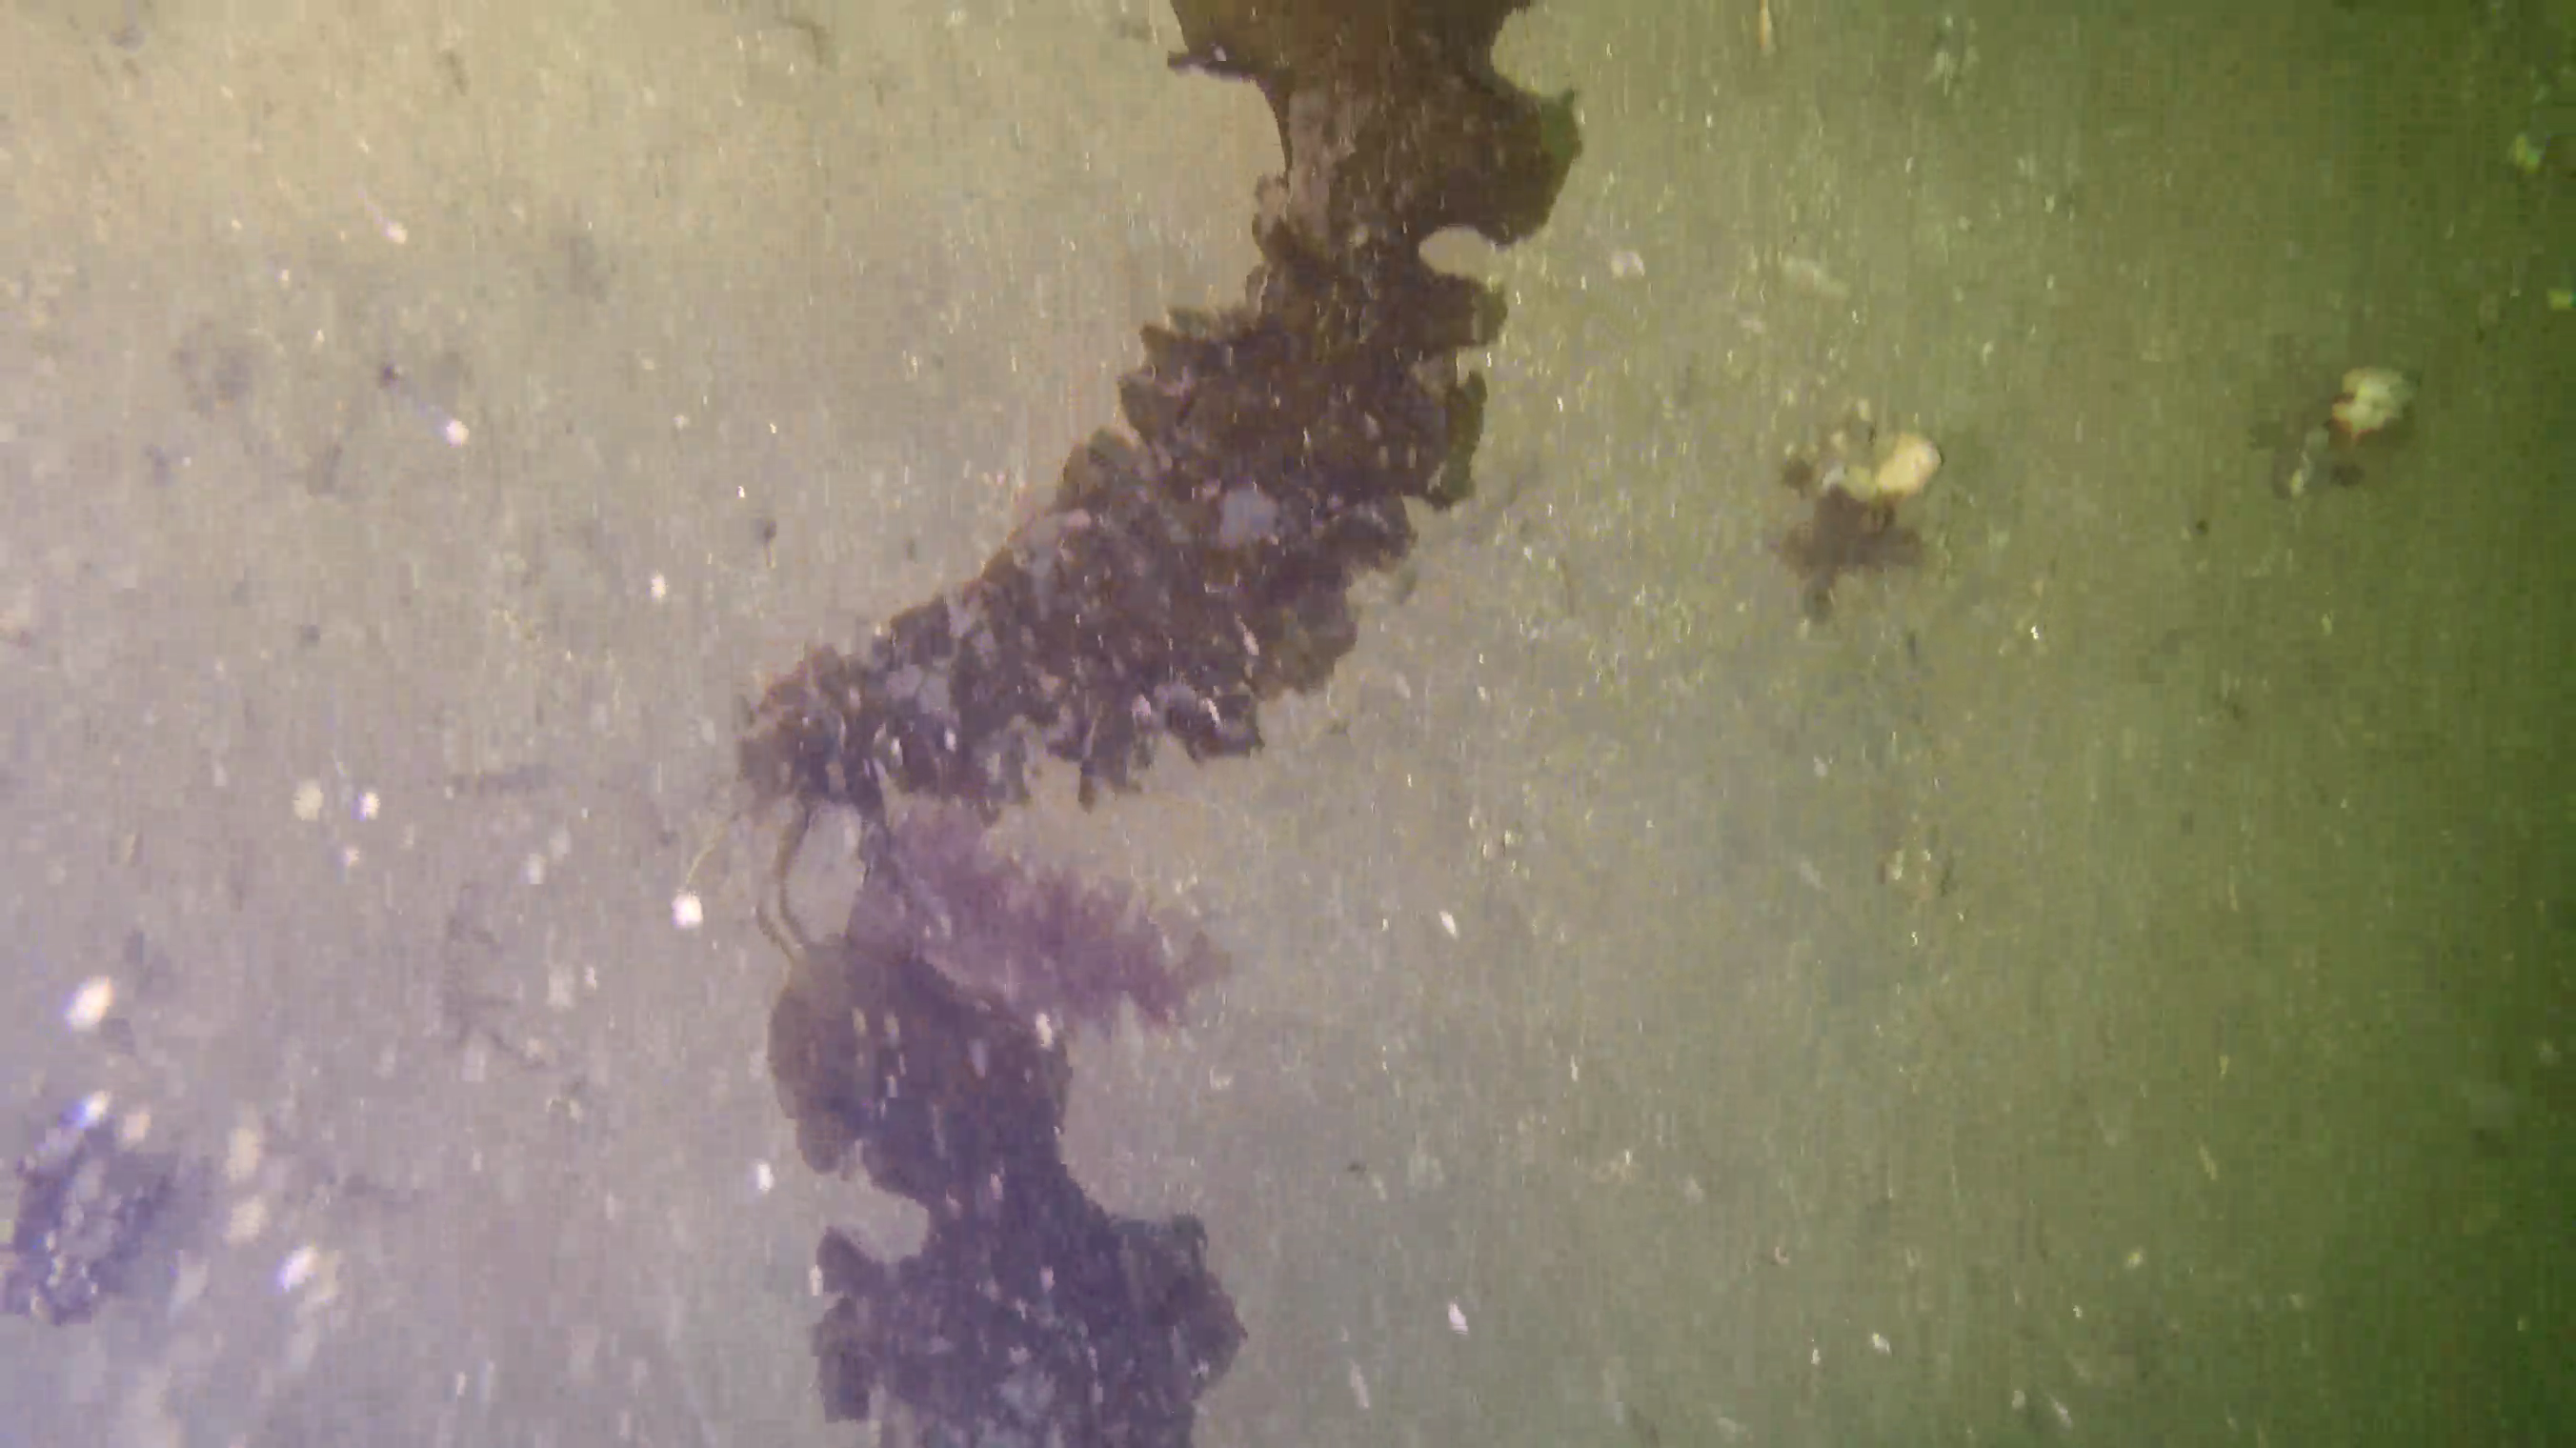
\includegraphics[width=1\linewidth]{assets/backscatter_test_vid.png}
        \caption{}
        % \label{subfig:backscatter_gopro}
    \end{subfigure}
    \caption{(a) Backscatter forms as the particles of sand drift between the aquatic animal and the camera \cite{brentdurandEasyWaysEliminate2013}. (b) A captured frame in GoPro footage from a UUV of the seabed with backscatter formed as the propellors disrupt the sand.}
    \label{fig:backscatter}
\end{figure}

The lack of light attenuation at greater sea depths is a critical challenge in underwater imaging, and to tackle this, an external high-power light source is often tied to a camera to ensure a well-lit scene. However, this produces an adverse side-effect: backscatter, shown in Figure \ref{fig:backscatter}, where suspended particles in water scatter light in an inhomogeneous manner, reflecting the light emitted by the light source back into the camera, creating exponentially bright spots and often saturating the image and degrading the quality. While there are a few simple and universal techniques to eliminate backscatter, such as reducing the separation between the subject and camera, fine-tuning the light source position such that only the edge of the light cone illuminates the subject, or achieving perfect buoyancy to minimise creating clouds of sand and debris \cite{brentdurandEasyWaysEliminate2013}, they lack viability for UUVs due to the erratic backscatter formation from the continuous and arbitrary motion of the propellors and general vehicular movement.

The ultimate goal of this project is to develop a novel light source system capable of aiding the generation of high-quality underwater images, of mainly the sea floor, from UUVs without backscatter interference. This project first aims to research systems and develop reliable backscatter detection and elimination capabilities, with a specialised projector serving as a dynamic light source of tailored light patterns for selective scene illumination to mitigate backscatter effects. The second research aim will look into architectures and methodologies to optimise the system for real-time to ensure adherence to stringent requirements for predictability, stability, efficiency, and reliability, ultimately allowing for imaging performance control in dynamic underwater environments whilst maintaining requirements. The final research aim is delving into the engineering of a predictive system for anticipating the future positions of detected backscatter particles, enabling proactive elimination strategies without the need for continuous, computationally intensive machine vision processing, for efficient and preemptive adjustments to the light projection patterns for optimal backscatter suppression. These three aims represent critical trade-offs that must be carefully balanced to achieve the overarching objective, which this research project aims to establish through systematic exploration and optimisation to lead towards a cutting-edge framework for enhancing underwater imaging capabilities.

This initial report forms a snapshot-based progress update on the project status. With the outline of the ultimate project goal and the aims, the report aims to summarise the background information in related theoretical realms considered thus far in the next section. The compiled background information will form the foundation of the subsequent sections, a discussion on the specifications to achieve the project goals with detail on hardware and software choices and a description of the intended project progression approach exemplified by a project schedule. Finally, a conclusion will close this report with a summary of details and any further thoughts.
